\newpage
\section{Caso 1.b, resistencia interna de la fuente 100k \texorpdfstring{$\Omega$}{ohm}}

Para este caso, las especificaciones indican que la resistencia interna de la fuente de señal es igual a 100k $\Omega$. Por lo tanto, para no cargar la fuente de señal, la impedancia debe ser mucho mayor a este valor, tomamos como criterio que sea 10 veces mas grande.

Luego, los requerimientos de diseño indican que debe tener una ganancia de -30 veces. 
ganancia vo a cada fuente de señal debe ser -30, 

\[ \text { Si: } R_{i}=100k \Omega \Longrightarrow R=10 \cdot R_{i} = 1 M\Omega \]
\[ \text { Cumpliendo la condición de }: \quad A_{vm} =-\frac{R_{f}}{R}=-30 \]
\[ \text { Obtenemos }: \quad R_{f}=30 M\Omega \]
Pero esto no cumple con el requerimiento de valor de impedancias menor a 1 M$\Omega$
\vspace{1em}

Por lo tanto debemos buscar una manera de obtener una impedancia de realimentación equivalente a 30 M$\Omega$ pero solo con resistores menores a 1 M$\Omega$.

Hay una forma, desviando utilizando un cuadripolo en ``T'' como realimentación y obtener el mismo resultado:


\begin{figure}[h!]
    \centering
    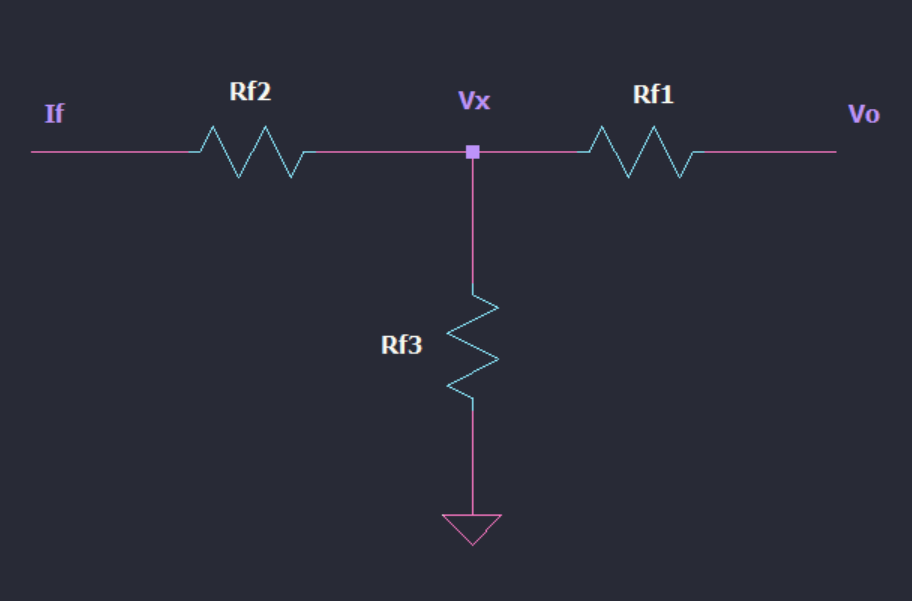
\includegraphics[width=1\linewidth]{img/cuadripoloT.png}
    \caption{Cuadripolo T equivalente a Rf}
    \label{fig:cuadripoloT}
\end{figure}

La impedancia de realimentación equivalente es igual a 

\[Rf = \frac{V_o}{I_f}\]

Para simplificar el calculo, vamos a considerar AO ideal, por lo que la entrada inversora va a ser igual a 0[V].

Luego podemos calcular Vx como la tensión sobre $R_{f3}$:

\[ V_x = \frac{  R_{f2} //  R_{f3} }{ R_{f2} //  R_{f3} + R_{f1} } V_0  = ... = \frac{R_{f2} R_{f3}}{R_{f1} (R_{f2} + R_{f3}) + R_{f2} R_{f3}} \cdot V_o
\]

Con la tensión $V_x$ podemos calcular la corriente $I_f$:

\[ I_f = \frac{V_x}{R_{f2}} = \frac{R_{f3}}{R_{f1} (R_{f2} + R_{f3}) + R_{f2} R_{f3}} \cdot V_o\]


Luego con esto podemos encontrar la impedancia $R_f$:

\[R_f = \frac{V_0}{V_x} \cdot \frac{V_x}{I_f} = \frac{R_{f1} (R_{f2} + R_{f3}) + R_{f2} R_{f3}}{R_{f3}} \]

\[R_f = \frac{R_{f1} \cdot R_{f2} }{R_{f3} } +R_{f1}  + R_{f2}  \]

Por medio de un método iterativo, y variando los valores de $R_{f1}$ y $R_{f2}$ se calcula un valor para $R{f3}$. Teniendo en cuenta valores normalizados de resistores.

\vspace{1em}

Como $R_f = 30M\Omega$ entonces elegimos un valor de $R_{f1} = 390k \Omega$ , $R_{f2} = 91k \Omega$ entonces calculamos:

\vspace{1em}
\[R_{f3} = 1202k\Omega \approxeq 1,2k \Omega \]


\begin{figure}[h!]
    \centering
    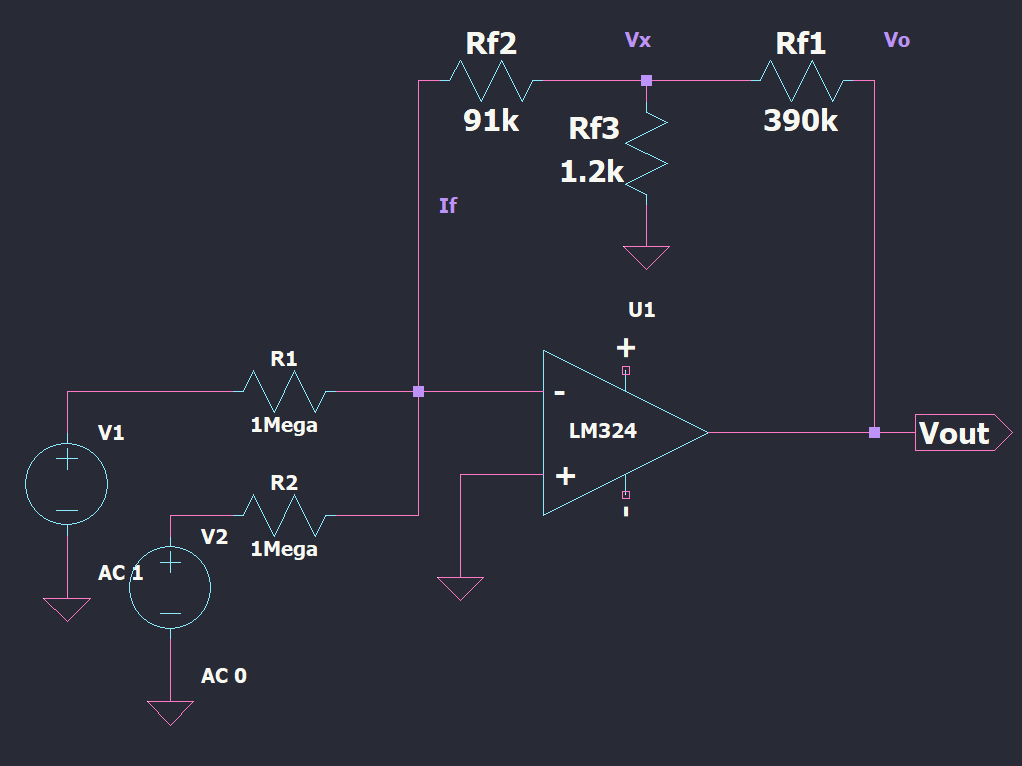
\includegraphics[width=0.90\linewidth]{img/caso1b.png}
    \caption{Esquemático para el caso 1b}
    \label{fig:caso1b}
\end{figure}


\[  \mathbf{R}=1M \Omega, \quad \mathbf{R}_{\mathbf{f}}=30M \mathrm{k} \Omega \]


De esta manera nuestro diseño cumple con las especificaciones de ganancia, impedancia de entrada y valor máximo de resistencias.

\vspace{1em}

\subsection{Errores en DC.}
En primer lugar, obtenemos todos los datos necesarios de la hoja de datos de la figura \ref{fig:caracteristicas}.

\vspace{1em}

Reemplazamos por los valores típicos, en las expresiones tenemos que:


\[V_{0} = -30 \cdot (V_1 + V_2) \]

Luego debemos recalcular T:

\[T = - Ad   \cdot  \frac{R \cdot R_{f3}}{ 2 \cdot (\frac{R}{2} + R_{f2})\cdot (R_{f1}+R_{f3})} = 3114,2 \]


\vspace{1em}

Para realizar los demás cálculos , consideramos a $R_{eq} = R_{f2} + R_{f3}//R_{f1} \approxeq 92k \Omega$
 
\[ \Delta V_{ios} = I_{pol}^{-} \cdot R_{eq} = 20 nF \cdot 92 k\Omega = 1,84 mV \]

\vspace{1em} 

\[ \Delta V_{os}  = V_{os} \cdot (1 + 2 \cdot \frac {R_{eq}}{R})  \approxeq
3mV \cdot 1,18 = 3,553 mV \]

\vspace{1em}

\[ \Delta V_{o (Ad)}=\frac{F.S}{\left|T_{o}\right|} = \frac{10V}{3114,2} = 0,8 mV\]

\vspace{1em}

\[ \Delta V_{o (RRMC) } = 0 [ mV ]\]

El error total DC es igual a:

\[ \Delta V_{O} = \Delta V_{ios} + \Delta V_{os} +  \Delta V_{o (A_d)} + \Delta V_{o (RRMC) } = 6,19 [mV]\]


\subsection{Errores en AC}
 
\subsubsection{Ancho de banda:}

 Primero obtenemos los valores correspondiente a nuestro amplificador de la hoja de datos. Luego
 
\[ f_H = f_{T} \frac{R}{R+2 R_f} = 1,2 [MHz] \cdot \frac{500}{30500} = 19,67 [kHz] \]

\subsubsection{Ancho de banda de potencia para 10 \texorpdfstring{$V_{pap}$}{Vpap}:}
\[ f_{Hp}=7,957[\mathrm{kHz}] \]

  
 
\newpage

\subsection{Simulaciones}
\subsubsection{Simulación de salida en el tiempo}
 
\begin{figure}[h!]
    \centering
    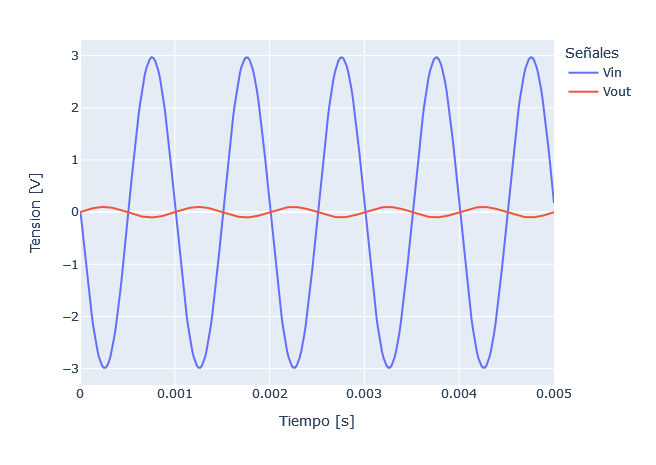
\includegraphics[width=0.80\linewidth]{img/TP2_1_grafico_tiempo}
    \caption{Gráfico de voltaje de salida en el tiempo}
    \label{fig:1b_tiempo}
\end{figure}

En esta simulación se puede observar que con una entrada de 100 [mV] a 1 [kHz] obtenemos aproximadamente 3[V] de salida. Al igual que la tensión de offset que tiene, ya que no inicia exactamente en 0[V].

\subsubsection{Simulación de barrido en frecuencia (bode)}

\begin{figure}[h!]
    \centering
    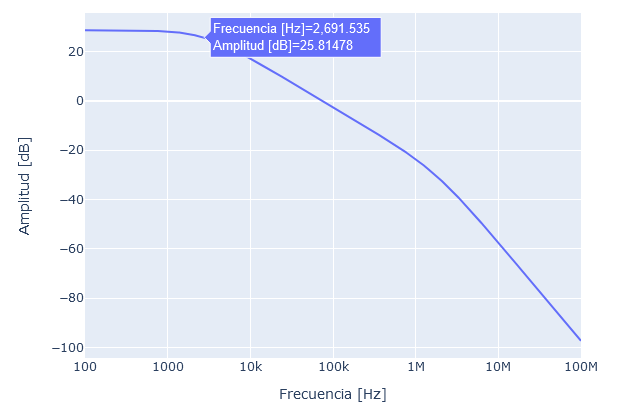
\includegraphics[width=0.80\linewidth]{img/TP2_2_grafico_bode_amp.png}
\end{figure}

\begin{figure}[h!]
    \centering
    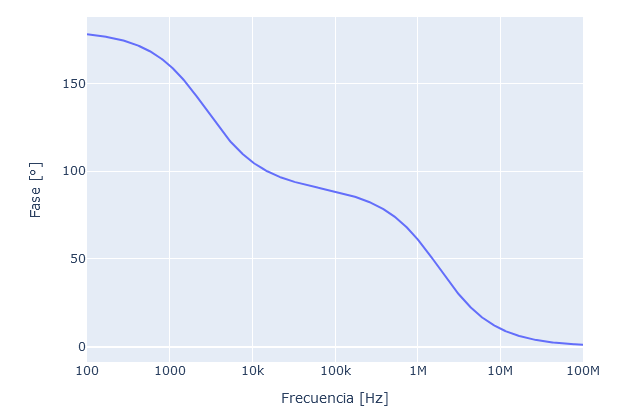
\includegraphics[width=0.80\linewidth]{img/TP2_2_grafico_bode_fase.png}
    \caption{Gráfico de barrido en frecuencia}
    \label{fig:bode}
\end{figure}

\subsubsection{Análisis en frecuencia }

Se pueden observar las armónicas de la señal de salida, frente a una señal de entrada de 1kHz.
\begin{figure}[h!]
    \centering
    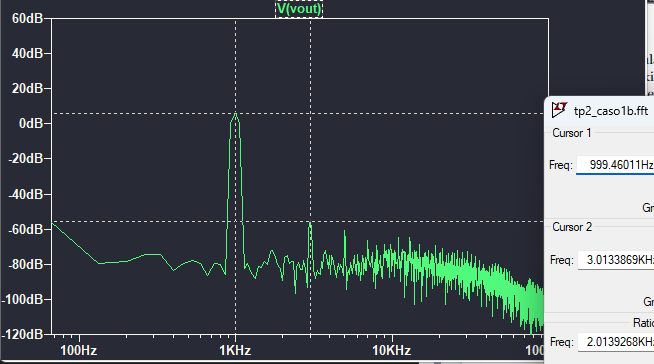
\includegraphics[width=0.80\linewidth]{img/ftt.png}
    \caption{Gráfico de la transformada de fourier}
    \label{fig:fft}
\end{figure}

\subsubsection{Simulación de entrada/salida}

En este caso realizamos un barrido en DC desde -2V a 2V para la fuente de señal $V_1$ y luego se gráfico la tensión de salida $V_o$:

A través de esta simulación se puede observar que la tensión máxima a la que llega la salida es 8,82[V]. Esto se debe a que el amplificador no es Rail to Rail. 

Tambien verificamos que la ganancia es aproximadamente igual a 30 veces.

\begin{figure}[h!]
    \centering
    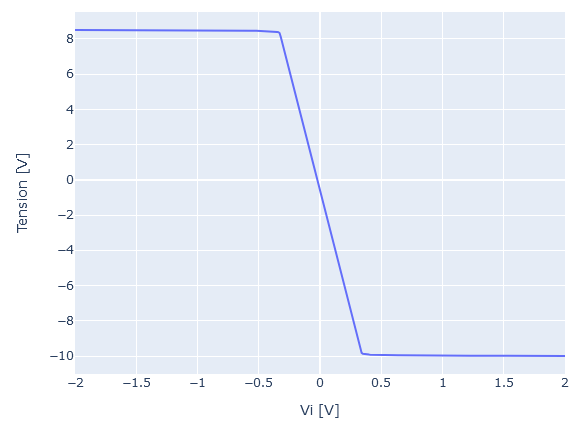
\includegraphics[width=0.80\linewidth]{img/TP2_2_grafico_entrada_salida.png}
    \caption{Gráfico Vo con respecto a Vi}
    \label{fig:vo_vi}
\end{figure}

\vspace{1em}

\subsubsection{Simulación del Slew rate }

Para esta simulación se puso como entrada una señal cuadrada con tiempo de subido de 1[pS], periodo de 1 [mS] y dutty cycle del 50\%. 

\begin{figure}[h!]
    \centering
    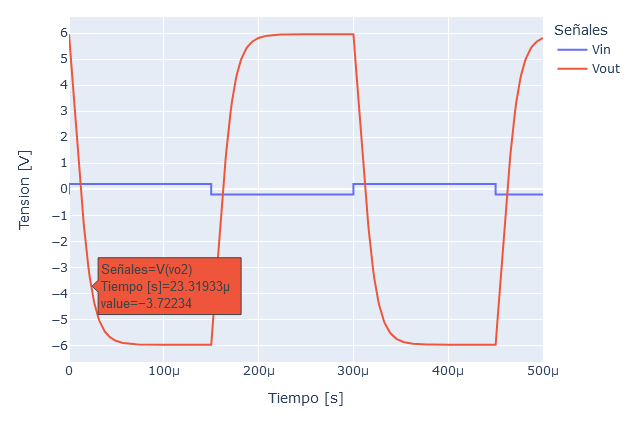
\includegraphics[width=0.90\linewidth]{img/TP2_2_grafico_slew.png}
    \caption{Gráfico del slew rate}
    \label{fig:1b_slew_rate}
\end{figure}


